\documentclass[../main.tex]{subfiles}
\begin{document}
\section*{Huffman Codes}
A simple constrution of optimal prefix codes.
\begin{itemize}
    \item Binary case: keep merging the 2 smallest probability masses until one probability mass (1) is left.
    \item D-ary Case: Insert zero probability masses until there are $D+k(D-1)$ masses, if necessary. Then keep merging the $D$ smallest probability masses until one probability mass is left.
    \item In general, there can be more than one Huffman code.
\end{itemize}
\begin{pbox}{Huffman Procedure}
    \begin{align*}
        p=\{0.35, 0.1, 0.15, 0.2, 0.2\}
    \end{align*}
    First we merge the 2 smallest probability masses to get \[
    p=\{0.35, 0.25, 0.2, 0.2\}
    \]. Then \[p=\{0.35, 0.25, 0.4\}\].
    Then \[p=\{0.6, 0.4\}.\]
    By doing so, we have formed a code tree. Assign the codes by the convention that going up appends $0$ and going down appends $1$.
\end{pbox}
\begin{bbox}{Lemmas for Optimality of Huffman Codes}
    Without loss of generality, assume $p_1\geq p_2\geq\dots \geq p_m,$ Denote the codeword assigned to $p_i$ by $c_i$ and its length by $l_i.$
    \begin{lemma}
        In an optimal code, shorter codewords are assigned to larger probabilities.
        \begin{proof}
            The expected length is improved (shortened) by swapping the a bad pair.
        \end{proof}
    \end{lemma}
    \begin{lemma}
        There exists an optimal code in which the codewords assigned to the 2 smallest probabilities are siblings (of same length and only differ in the last symbol.)
        \begin{proof}
            From the above lemma, the codeword $c_m$ has the longest length because it has the smallest probability. Then the sibling of $c_m$ canot be the prefix of another codeword. \\
            The sibling of $c_m$ must be a codeword because: otherwise, we replace $c_m$ by its parent to improve the code, contradicting the optimality of the code.
        \end{proof}
    \end{lemma}
\end{bbox}
Here we introduce the concept of reduced code tree: suppose $c_i$ and $c_j$ are siblings in a code tree, if we merge them into their comman parent called $c_{ij}$ and also merge the probabilities into $p_i+p_j$, we will imrove the expected codeword length by $p_i+p_j$.\\
Note this improvement only depends on the distribution over the words but not the structure of the reduced code tree.
\begin{bbox}{Optimality of Huffman Procedure}
\begin{proof}
    Recursive proof: Consider an optimal code in which $c_m$ and $c_{m-1}$ are siblings. Existence by lemma.\\
    Let $p'$ be the reduced distribution by merging $p_m$ and $p_{m-1}$. Let $L$ and $L'$ be the expected word lengths of the original and reduced code respectively.\\
    \[
    L = L' + (p_{m-1} + p_m).
    \]
    So $L$ is the optimal length for $p$ if and only if $L'$ is the optimal length for $p.$\\
    Reduce the problem all the way to 2 probability masses, for which optimal code is easy to find. 
\end{proof}
\end{bbox}
The idea for D-ary Huffman Procedure is similar.
\begin{bbox}{Upper Bound of the optimal codeword length!}
    The expected length of a Huffman code, denoted by $L_{Huff}$, satisfies the inequality \[
    L_{Huffman} < H_D(X)+1
    \]
    This is the tightest bound among all upper bounds on $L_{Huff}$ which depends only on the source random variable's entropy.
    \begin{proof}
        Construct a code with codeword lengths $l_i=\lceil -\log_{D}p_i\rceil$ and show that the Kraft inequality is satisfied. \[
        -\log p_i \leq l_i < -\log p_i + 1
        \]\[
        \log p_i \leq l_i > \log p_i - 1
        \]\[
        p_i \geq D^{-l_i} \geq D^{-1}p_i
        \]
        \[
        \sum_i D^{-l_i} \leq \sum_{i}p_i = 1
        \]. So prefix code exists.
        Then $L=\sum_i p_i l_i < H(X)+1$.\\
        Lastly, use the fact that $L_{Hugg}\leq L$ by optimality.\\
        To show this is the tightest bound, we have to show that $H_D(X)+1$ can be achieved as a limit of a sequence of $L_{Huff}$s. 
        Such sequence can be chosen as follows: \[
        p_k=\{1-\frac{D-1}{k},\frac{1}{k},\dots,\frac{1}{k}\} \quad\text{(D-1) copies of $\frac{1}{k}$}.
        \] As $k$ goes to infinity, the entropy goes to $0$. The Huffman code for each $p_k$ consists of $D$ codewords length $1$.
    \end{proof}
\end{bbox}
\begin{bbox}{Asymptotic Achievability of $H(X)$}
\[
    H(X)\leq L_{Huff} < H(X)+1
\]
If we use a Huffman code to encode $n$ i.i.d. copies of $X$. Then \[
    nH(X)\leq L^{n}_{Huff} < nH(X)+1
\] 
Then \[
H(X)\leq \frac{1}{n}L^{n}_{Huff} < H(X)+\frac{1}{n}\to H(X)
\] as $n\to \infty$
$\frac{1}{n}L^{n}_{Huff}$ is called the \textbf{rate} of the code, measured in $D$-it per source symbol.
This is the average number of $D-ary$ symbols to encode a source symbol(RV)
\begin{remark*}
    Therefore, in asymptotic sense, the entropy $H(X)$ measures the amount of information contained in $X$.
\end{remark*}
\end{bbox}

\section*{Redundancy of Prefix Codes}
In previous section, we have proved the entropy bound for a $D-ary$ uniquely decodable code \[
L\geq H_D(X)
\]
We now prove this bound specially for prefix code and this will offer insights about the redundancy of a code.
\centering{\textbf{A D-ary Code Tree}}
\begin{itemize}
    \item Let $X$ be a source random variable with probability distribution $\{p_1,\dots,p_m\}$
    \item A D-ary prefix code for $X$ can be represented by a $D-$ary code tree with $m$ leaves, where each leaf corresponds to a codeword.
    \item Ddenote the leaf (word) corresponding to $p_i$ by $c_i$
 and the order of $c_i$ by $l_i$ (length)
 \item Let the alphabet be $\{0,\dots,D-1\}$.
 \item Let $\I$ be the index set of all the internal codes (including the root) in the code tree. (a node that has at least one descendant.)
 \end{itemize}
 \centering{\textbf{Reaching Probability}}
 \begin{itemize}
     \item To decode codeword of a prefix code, we can trace the path specified by the codeword from the root of the code tree until it terminates at the leaf corresponding to that codeword.
     \item Let $q_k$ be the probability of reaching an internal node $k$ during the decoding process.
     \item $q_k$ is equal to the sum of the probabilities of all the leaves decending from node $k$.
 \end{itemize}
 \centering{\textbf{Branching at an Internal Node}}
 \begin{itemize}
     \item Let $p_{k,j}$ be the probability that the $j$th branch of node $k$ is taken during the decoding process.
     \item The probabilities $p_{k,j}$ where $0\leq j\leq D-1$, are called the branching probabilities of node $k$, and \[
     q_k = \sum_j p_{k,j}
     \]
     \item Once node $k$ is reached, the conditional branching distribution is \[
     \{\frac{p_{k,0}}{q_k},\dots,\frac{p_{k,D-1}}{q_k}\}
     \],
     obtained by normalizing $p_{k,\cdot}$
     \item Then define the conditional entropy of node $k$ by \[
     h_k = H_D(\{\frac{p_{k,0}}{q_k},\dots,\frac{p_{k,D-1}}{q_k} \}) = \leq \log_D D = 1
     \]
 \end{itemize}
 \begin{bbox}{4.19 A Lemma}
     \[
     H_D(X)=\sum_{k\in \I}q_k h_k
     \] where \begin{itemize}
         \item $q_k$ is the reaching probability of internal node $k$
         \item $h_k$ is the conditional entropy of internal node $k$.
     \end{itemize}
     \begin{proof}
         Induction on the number of internal nodes.\\
         For the base case, if there is only one internal node, it must be the root of the code tree. Then the lemma is trivially true because the reaching probability of the root is $1$ and all the codewords have length of $1$\\
         Now inductive step: assume the lemma is true for code trees with $n$ internal nodes. Let $k$ be an internal code such that it is the parent of a leaf $c$ with maximum order.\\
         Each sibling of $c$ may or may not be a leaf. If it is not a leaf, it cannot be the ascendant of another leaf, otherwise contradicting the maximality of the order of $c$. \\
         Now consider revealing the outcome of $X$ in 2 steps. In the first step, if the outcome of $X$ is not a leaf descending from $k$, we identify the outcome exactly, otherwise we identify the outcome to be a child of node $k$. We call this random variable $V$.\\
         If we do not identify the outcome exactly in the first step, which happens with probability $q_k$, we further identify in the second step which of the children of node $k$ the outcome is. We call this random variable $W$.\\
         Then $X=(V,W)$.
         The outcome of $V$ can be represented by a code tree with $n$ internal nodes which is obtained by prunning the original code tree at node $k$.
         By the inductive hypothesis, 
         Then \[
         H(X)=H(V,W)=H(V)+ H(W|V)
         \]
     \end{proof}
 \end{bbox}
 \begin{bbox}{4.20 Expected Length in terms of $q_k$}
     \[
     L = \sum_{k\in\I}q_k
     \]
     \begin{proof}
         Easy to show by drawing a tree.\\
         Rigorously, we can define a quantity \[a_{ki}=\begin{cases}
             1 \quad \text{if leaf $c_i$ is a descendent of internal node $k$}\\
             0 \quad \text{otherwise}
         \end{cases}\]
     \end{proof}
 \end{bbox}
 \centering{\textbf{Local Redendancy}}
 \begin{itemize}
     \item Define the local redundancy of an internal node $k$ by \[
     r_k = q_k(1-h_k)
     \]
     \item This quantity is local wrt note $k$ in the sense that it only depends on the branching probabilities of node $k$.
     \item $r_k=0$ if and only if \[
     p_{k,j}=\frac{q_k}{D}
     \] for all $j$, i.e. if and only if the internal node $k$ is \textbf{balanced}.
 \end{itemize}
 \begin{bbox}{Local Redundancy Theorem}
     Let $R$ be the redundancy of a D-ary prefix code for a source random variable $X$. Then \[
     R=\sum_{k\in\I}r_k
     \]
     \begin{proof}
         \begin{align*}
             R &= L - H_D(X)\\
             &= \sum_{k}q_k - \sum_{k}q_kh_k\\
             &= \sum r_k
         \end{align*}
     \end{proof}
 \end{bbox}
\begin{bbox}{Entropy Bound for Prefix Code}
Let $R$ be the redundancy of a prefix code. Then $R\geq 0$ with equality if and only if all the internal nodes in the code tree are balanced.
\begin{proof}
    Consider \[
    R=\sum_{k\in \I}r_k.
    \]
    $R \geq 0$ is non-negative because $r_k\geq 0$ for all internal nodes $k$.\\
    $R=0$ if and only all $r_k$ are $0$, meaning all of the internal nodes are balanced.
\end{proof}
\end{bbox}
\begin{itemize}
    \item The entropy bound says that $H_D(X)\leq L$. 
    \item This makes sense because intuitively each $D-ary$ symbol can carry at most $1$ D-it of information.
    \item Therefore, when the entropy bound is tight, each code symbol has to carry exactly one $D-it$ of information.
    \item InterpretationL Consider revealing a a random variable codeword one symbol at a time. Balanced: as long as the codeword is not completed, the next code symbol to be revealed always carries one $D-it$ of  information because it is distributed uniformly on the alphabet.
\end{itemize}
Now we discuss a lower bound on $R$. Consider \[
R=\sum_{k\in \I}r_k \geq \sum_{k\in \I'}r_k
\] for any subset $\I'$ of $\I$.\\
If we can compute $r_k$ for all $k\in \I'$, we can compute a lower bound.


\chapter{Weak Typicality}
We will discuss\begin{itemize}
    \item for $X=(X_1,X_2,\dots,X_n)$ where $X_i$ are i.i.d. $\sim p(x)$, what a "typical" outcome of $X$ would be.
    \item How typical sequences are related to data compression.
    \item Shannon's source coding theorem for data compression.
\end{itemize} 

\section{The Weak AEP}
\centering{\textbf{The Notion of Typical Sequences}}
Consider tossing a fair coin $n$ times. If the outcome is "head" approximately half of the time, the sequence of outcome is "normal" or "typical." How to quantify the typicality of a sequence?\\
Answer: weak and strong typicality.\\
The main theorems are weak and strong Asymptotic Equipartition Properties (AEP), consequences of weak law of large numbers.
\centering{\textbf{Setup}}
\begin{itemize}
    \item $\{X_k,k\geq 1\}$, $X_k$ iid $\sim p(x)$.
    \item $X$ denotes generic rv with finite entropy.
    \item Let $\mathcal{X}=(X_1,\dots,X_n)$, then $p(\vec X=p(X_1)\dots p(X_n).$
    \item The alphabet $\X$ is allowed to be countably infinite.
    \item Let the base of log be 2, so the unit of entropy $H(X)$ is  bit.
\end{itemize}
Note that in Cover's textbook, the weak AEP is just called AEP.
\begin{bbox}{Weak AEP I}
    \begin{equation*}
        -\frac{1}{n}\log p(X_1,...X_n)\to H(X)
    \end{equation*} in probability as $n\to\infty$.\\
    For any $\epsilon>0$,\[
    \lim_{n\to\infty}P\{|-\frac{1}{n}\log p(X_1,...,X_n) - H(X)|>\epsilon\}=0.
    \]
    Another way to say this is: \[
    P\{|-\frac{1}{n}\log p(X_1,...,X_n) - H(X)| \leq \epsilon\} > 1-\epsilon
    \]
    \begin{proof} Quick consequence of weak law of large numbers. By independence, $p(X_1,...,X_n)=p(X_1)\dots p(X_n)$. Then log of product is equal to sum of logs. Then sum becomes the sample mean.
    \end{proof}
\end{bbox}
\begin{gbox}{Weakly typical set}
    The weakly typical set $W^n_{X_\epsilon}$ with respect to $p(x)$ is the set of sequences $\vec x=(x_1,\dots,x_n)\in \X^n$ such that \[|-\frac{1}{n}\log p(\vec x)-H(X)| \leq \epsilon\], or equivalently \[
    H(X)-\epsilon \leq -\frac{1}{n}\log p(\vec x)\leq H(X)+\epsilon.
    \]
    The sequences in $W$ are called wealy $\epsilon-$typical sequences. 
\end{gbox}
\begin{gbox}{Empirical Entropy}
    The empirical entropy of a sequence $\vec x = (x_1,...,x_n)$ is defined as \begin{equation*}
        -\frac{1}{n}\log p(\vec x)=-\frac{1}{n}\log \Pi_{k=1}^np(x_k) = -\frac{1}{n}\sum_{k=1}^n \log p(x_k)   \end{equation*}
    A typical sequence is just a sequence whose empirical entropy is close to the true entropy $H(X)$.
\end{gbox}
\begin{bbox}{Weak AEP II}
For any $\epsilon > 0$:
\begin{itemize}
    \item If $\vec x\in W$, then \[
    2^{-n(H(X)+\epsilon)}\leq p(\vec x)\leq 2^{-n(H(X)-\epsilon)}
    \]
    \item For n sufficiently large, \[
    P(\vec X\in W) > 1-\epsilon.\]
    \item For n sufficiently large, \[
    (1-\epsilon)2^{n(H(X)-\epsilon)}\leq |W|\leq 2^{n(H(X)+\epsilon)}
    \]
    
\end{itemize}
\begin{proof}
    \begin{enumerate}
        \item The first bullet point is simply multiplying both sides of the equation in the definition of by $n$ and then take exponential.
        \item Re-expression of the same event.
        \item From the first point, we get a lower bound on $p(\vec x)$, then $|W|\cdot 2^{-n(H(X)+\epsilon)} \leq P(W)\leq 1$
    \end{enumerate}
\end{proof}
\end{bbox}
Weak AEP says that 
\begin{itemize}
    \item For large $n$, the probability of occurrence of the sequence drawn is close to $2^{-nH(X)}$ with high probability. The probabilities of the typical sequences are almost the same.
    \item The total number of weakly typical sequences is approximately equal to $2^{nH(X)}$.
\end{itemize}
However, Weak AEP does NOT say that most sequences are weakly typical. It also does NOT  say that the most likely sequences is weakly typical.
\begin{pbox}{Example}
    Consider $X$ such that $p(0)=0.2$ and $p(1)=0.8$.
    \begin{itemize}
        \item The most likely sequence is $\vec 1 = (1,1,\dots, 1)$ with $p(\vec 1) = 0.8^n$.
        \item Then \[-\frac{1}{n}\log p(\vec 1)=-\frac{1}{n}\log 0.8^n =-\log 0.8\neq H(X)    
        \], not close to true entropy, so $\vec 1$ is not typical.
        \item This seems to be a contradiction because $P(W)\approx 1$ but $\vec 1\notin W$. This is actually not a contradiction because $p(\vec 1)\to 0$.x
        \end{itemize}
\end{pbox}
When $n$ is large, one can think of the sequence $\vec X$ as being obtained by choosing a sequence from the weakly typical set uniformly at random! (because the probabilities of the typical sequences are almost the same)\\
Note $|W|\approx 2^{nH(X)}$.\[
2^{nH(X)} << 2^{n\log |\X|}= |\X|^n=|X^n|
\]
Therefore the size of the typical set would be much smaller than the size of all possible sequences., while having almost all the probability mass.

\section{The Source Coding Theorem}
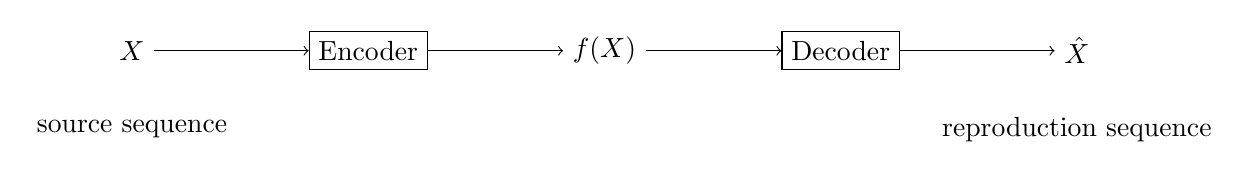
\begin{tikzpicture}[node distance=2cm,auto]
    % Nodes
    \node (source) {$X$};
    \node [below of=source, node distance=1cm] {source sequence};
    \node [right of=source, draw, rectangle, node distance=3cm] (encoder) {Encoder};
    \node [right of=encoder, node distance=3cm] (f) {$f(X)$};
    \node [right of=f, draw, rectangle, node distance=3cm] (decoder) {Decoder};
    \node [right of=decoder, node distance=3cm] (reproduction) {$\hat{X}$};
    \node [below of=reproduction, node distance=1cm] {reproduction sequence};

    % Arrows
    \draw [->] (source) -- (encoder);
    \draw [->] (encoder) -- (f);
    \draw [->] (f) -- (decoder);
    \draw [->] (decoder) -- (reproduction);
\end{tikzpicture}\\
\begin{itemize}
    \item The encoder maps a random source sequence $\vec X\in \X^n$ to an index $f(\vec X)$ in an index set $\{1,2,\dots,M\}$.
    \item Such a code is called a block code with block length $n$.
    \item The encoder sends $f(\X)$ to the decoder through a noiseless channel.
    \item Based on the index, the decoder outputs $\hat{\vec X}$ as an estimate on $\vec X$.
    \item The encoder is specified by $f:\X^n\to \{1,...,M\}$
    \item The rate of the code is given by $R=n^{-1}\log M$ in bits per source symbol, where $M$ is the size of the index set and $n$ is the block length. 
    \item If $M=|\X^n|$, the rate of the code is $\log |\X|$.
    \item Typically, we take $R < \log |\X|$ for data compression. Notice that because the number of indices is less than the total number number of sequences, the decoder may not be able to reproduce the source sequence correctly.
    \item Denote the error probability by $P_e := P(\vec X\neq \hat{\vec X})$
\end{itemize}
\begin{bbox}{The Source Coding Theorem}
    For arbitrarily small $P_e$, there exists a block code whose coding rate is arbitrarily close to $H(X)$ when $n$ is sufficiently large.
    \begin{itemize}
        \item This direction says that reliable communication can be achieved if the coding rate at least $H(X)$.
    \end{itemize}
    For any block code with block length $n$ and coding rate less than $H(X)-\zeta$, where $\zeta >0$ does not change with $n$, then $P_e\to 1$ as $n\to \infty$.
    \begin{itemize}
        \item This says it's impossible to achieve reliable communication if the coding rate is less than $H(X)$.
    \end{itemize}
    \begin{proof}
    
        For the first part, we need to construct a sequence of codes with block length $n$ such that $P_e < \epsilon$ for large $n$. \\

        \begin{remark}
            The idea is to choose a subset $A$ of $\X^n$ and let $M=|A|$. For each sequence $\vec x$ in $A$, assign it to a unique index $f(\vec x)$. For each source sequence $\vec x\notin A$, just let $f(\vec 1)$.\\
            For the decoding, if $\vec x \in A$, we are good. If not, then the decoding fails, so \[
            P_e = P(\vec X\notin A)
            \] 
        \end{remark}
        For $\epsilon > 0$, consider the $\epsilon$-typical set $W_\epsilon$, and we take $M=|W|$\\
        For sufficiently large n, the size of the $W$ is close to $2^{n(H(X))}$\\
        The coding rate satisfies $\frac{1}{n}\log(1-\epsilon) + H(X)-\epsilon \leq \frac{1}{n}\log M \leq H(X)+\epsilon$,
        by Weak AEP, $P_e = P(\vec X\notin W)$. The coding rate tends to $H(X)$ and $P_e$ tends to $0$ as $\epsilon \to 0$.
        \newline
        For the second part, the idea is that the set $A$ covers part of the typical set.
    \end{proof}
\end{bbox}
\begin{bbox}{Source Coding Theorem Converse}
    For any block code with blcok length $n$ and coding rate less than $H(X)-\zeta$, where $\zeta>0$ does not change with $n$, then $P_\epsilon\to 1$ as $n\to \infty$.
    \begin{proof}
        \[
        rate = \frac{1}{n}\log M < H(X)-\zeta
        \] where $\zeta>0$ does not change with $n$. The total number of codewords \[
        M\leq 2^{n(H(X)-\zeta)}
        \]
        Some of the indices in our index set $\I$ cover $\vec x \in W_{\epsilon}$.\\
        By WAEP, the total probabilty of typical sequences is upper bounded by \[
        2^{n(H(X)-\zeta)}2^{-n(H(X))-\epsilon} = 2^{-n(\zeta - \epsilon)}
        \]
        \[
        P(\vec X \in A) \leq 2^{-n(\zeta - \epsilon)} + P(X\notin W_\epsilon) < 2^{-n(\zeta - \epsilon)} + \epsilon
        \]
        Let $\epsilon\to 0$, we see that the probability of not making mistake goes to $0$.
    \end{proof}
\end{bbox}
\end{document}